\documentclass[1p]{elsarticle_modified}
%\bibliographystyle{elsarticle-num}

%\usepackage[colorlinks]{hyperref}
%\usepackage{abbrmath_seonhwa} %\Abb, \Ascr, \Acal ,\Abf, \Afrak
\usepackage{amsfonts}
\usepackage{amssymb}
\usepackage{amsmath}
\usepackage{amsthm}
\usepackage{scalefnt}
\usepackage{amsbsy}
\usepackage{kotex}
\usepackage{caption}
\usepackage{subfig}
\usepackage{color}
\usepackage{graphicx}
\usepackage{xcolor} %% white, black, red, green, blue, cyan, magenta, yellow
\usepackage{float}
\usepackage{setspace}
\usepackage{hyperref}

\usepackage{tikz}
\usetikzlibrary{arrows}

\usepackage{multirow}
\usepackage{array} % fixed length table
\usepackage{hhline}

%%%%%%%%%%%%%%%%%%%%%
\makeatletter
\renewcommand*\env@matrix[1][\arraystretch]{%
	\edef\arraystretch{#1}%
	\hskip -\arraycolsep
	\let\@ifnextchar\new@ifnextchar
	\array{*\c@MaxMatrixCols c}}
\makeatother %https://tex.stackexchange.com/questions/14071/how-can-i-increase-the-line-spacing-in-a-matrix
%%%%%%%%%%%%%%%

\usepackage[normalem]{ulem}

\newcommand{\msout}[1]{\ifmmode\text{\sout{\ensuremath{#1}}}\else\sout{#1}\fi}
%SOURCE: \msout is \stkout macro in https://tex.stackexchange.com/questions/20609/strikeout-in-math-mode

\newcommand{\cancel}[1]{
	\ifmmode
	{\color{red}\msout{#1}}
	\else
	{\color{red}\sout{#1}}
	\fi
}

\newcommand{\add}[1]{
	{\color{blue}\uwave{#1}}
}

\newcommand{\replace}[2]{
	\ifmmode
	{\color{red}\msout{#1}}{\color{blue}\uwave{#2}}
	\else
	{\color{red}\sout{#1}}{\color{blue}\uwave{#2}}
	\fi
}

\newcommand{\Sol}{\mathcal{S}} %segment
\newcommand{\D}{D} %diagram
\newcommand{\A}{\mathcal{A}} %arc


%%%%%%%%%%%%%%%%%%%%%%%%%%%%%5 test

\def\sl{\operatorname{\textup{SL}}(2,\Cbb)}
\def\psl{\operatorname{\textup{PSL}}(2,\Cbb)}
\def\quan{\mkern 1mu \triangleright \mkern 1mu}

\theoremstyle{definition}
\newtheorem{thm}{Theorem}[section]
\newtheorem{prop}[thm]{Proposition}
\newtheorem{lem}[thm]{Lemma}
\newtheorem{ques}[thm]{Question}
\newtheorem{cor}[thm]{Corollary}
\newtheorem{defn}[thm]{Definition}
\newtheorem{exam}[thm]{Example}
\newtheorem{rmk}[thm]{Remark}
\newtheorem{alg}[thm]{Algorithm}

\newcommand{\I}{\sqrt{-1}}
\begin{document}

%\begin{frontmatter}
%
%\title{Boundary parabolic representations of knots up to 8 crossings}
%
%%% Group authors per affiliation:
%\author{Yunhi Cho} 
%\address{Department of Mathematics, University of Seoul, Seoul, Korea}
%\ead{yhcho@uos.ac.kr}
%
%
%\author{Seonhwa Kim} %\fnref{s_kim}}
%\address{Center for Geometry and Physics, Institute for Basic Science, Pohang, 37673, Korea}
%\ead{ryeona17@ibs.re.kr}
%
%\author{Hyuk Kim}
%\address{Department of Mathematical Sciences, Seoul National University, Seoul 08826, Korea}
%\ead{hyukkim@snu.ac.kr}
%
%\author{Seokbeom Yoon}
%\address{Department of Mathematical Sciences, Seoul National University, Seoul, 08826,  Korea}
%\ead{sbyoon15@snu.ac.kr}
%
%\begin{abstract}
%We find all boundary parabolic representation of knots up to 8 crossings.
%
%\end{abstract}
%\begin{keyword}
%    \MSC[2010] 57M25 
%\end{keyword}
%
%\end{frontmatter}

%\linenumbers
%\tableofcontents
%
\newcommand\colored[1]{\textcolor{white}{\rule[-0.35ex]{0.8em}{1.4ex}}\kern-0.8em\color{red} #1}%
%\newcommand\colored[1]{\textcolor{white}{ #1}\kern-2.17ex	\textcolor{white}{ #1}\kern-1.81ex	\textcolor{white}{ #1}\kern-2.15ex\color{red}#1	}

{\Large $\underline{12a_{0800}~(K12a_{0800})}$}

\setlength{\tabcolsep}{10pt}
\renewcommand{\arraystretch}{1.6}
\vspace{1cm}\begin{tabular}{m{100pt}>{\centering\arraybackslash}m{274pt}}
\multirow{5}{120pt}{
	\centering
	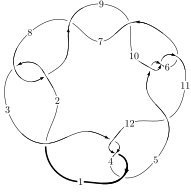
\includegraphics[width=112pt]{../../../GIT/diagram.site/Diagrams/png/1601_12a_0800.png}\\
\ \ \ A knot diagram\footnotemark}&
\allowdisplaybreaks
\textbf{Linearized knot diagam} \\
\cline{2-2}
 &
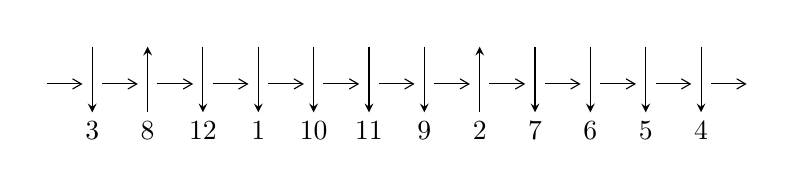
\begin{tikzpicture}[x=20pt, y=17pt]
	% nodes
	\node (C0) at (0, 0) {};
	\node (C1) at (1, 0) {};
	\node (C1U) at (1, +1) {};
	\node (C1D) at (1, -1) {3};

	\node (C2) at (2, 0) {};
	\node (C2U) at (2, +1) {};
	\node (C2D) at (2, -1) {8};

	\node (C3) at (3, 0) {};
	\node (C3U) at (3, +1) {};
	\node (C3D) at (3, -1) {12};

	\node (C4) at (4, 0) {};
	\node (C4U) at (4, +1) {};
	\node (C4D) at (4, -1) {1};

	\node (C5) at (5, 0) {};
	\node (C5U) at (5, +1) {};
	\node (C5D) at (5, -1) {10};

	\node (C6) at (6, 0) {};
	\node (C6U) at (6, +1) {};
	\node (C6D) at (6, -1) {11};

	\node (C7) at (7, 0) {};
	\node (C7U) at (7, +1) {};
	\node (C7D) at (7, -1) {9};

	\node (C8) at (8, 0) {};
	\node (C8U) at (8, +1) {};
	\node (C8D) at (8, -1) {2};

	\node (C9) at (9, 0) {};
	\node (C9U) at (9, +1) {};
	\node (C9D) at (9, -1) {7};

	\node (C10) at (10, 0) {};
	\node (C10U) at (10, +1) {};
	\node (C10D) at (10, -1) {6};

	\node (C11) at (11, 0) {};
	\node (C11U) at (11, +1) {};
	\node (C11D) at (11, -1) {5};

	\node (C12) at (12, 0) {};
	\node (C12U) at (12, +1) {};
	\node (C12D) at (12, -1) {4};
	\node (C13) at (13, 0) {};

	% arrows
	\draw[->,>={angle 60}]
	(C0) edge (C1) (C1) edge (C2) (C2) edge (C3) (C3) edge (C4) (C4) edge (C5) (C5) edge (C6) (C6) edge (C7) (C7) edge (C8) (C8) edge (C9) (C9) edge (C10) (C10) edge (C11) (C11) edge (C12) (C12) edge (C13) ;	\draw[->,>=stealth]
	(C1U) edge (C1D) (C2D) edge (C2U) (C3U) edge (C3D) (C4U) edge (C4D) (C5U) edge (C5D) (C6U) edge (C6D) (C7U) edge (C7D) (C8D) edge (C8U) (C9U) edge (C9D) (C10U) edge (C10D) (C11U) edge (C11D) (C12U) edge (C12D) ;
	\end{tikzpicture} \\
\hhline{~~} \\& 
\textbf{Solving Sequence} \\ \cline{2-2} 
 &
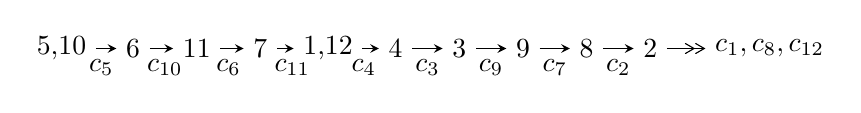
\begin{tikzpicture}[x=23pt, y=7pt]
	% node
	\node (A0) at (-1/8, 0) {5,10};
	\node (A1) at (1, 0) {6};
	\node (A2) at (2, 0) {11};
	\node (A3) at (3, 0) {7};
	\node (A4) at (65/16, 0) {1,12};
	\node (A5) at (41/8, 0) {4};
	\node (A6) at (49/8, 0) {3};
	\node (A7) at (57/8, 0) {9};
	\node (A8) at (65/8, 0) {8};
	\node (A9) at (73/8, 0) {2};
	\node (C1) at (1/2, -1) {$c_{5}$};
	\node (C2) at (3/2, -1) {$c_{10}$};
	\node (C3) at (5/2, -1) {$c_{6}$};
	\node (C4) at (7/2, -1) {$c_{11}$};
	\node (C5) at (37/8, -1) {$c_{4}$};
	\node (C6) at (45/8, -1) {$c_{3}$};
	\node (C7) at (53/8, -1) {$c_{9}$};
	\node (C8) at (61/8, -1) {$c_{7}$};
	\node (C9) at (69/8, -1) {$c_{2}$};
	\node (A10) at (11, 0) {$c_{1},c_{8},c_{12}$};

	% edge
	\draw[->,>=stealth]	
	(A0) edge (A1) (A1) edge (A2) (A2) edge (A3) (A3) edge (A4) (A4) edge (A5) (A5) edge (A6) (A6) edge (A7) (A7) edge (A8) (A8) edge (A9) ;
	\draw[->>,>={angle 60}]	
	(A9) edge (A10);
\end{tikzpicture} \\ 

\end{tabular} \\

\footnotetext{
The image of knot diagram is generated by the software ``\textbf{Draw programme}" developed by Andrew Bartholomew(\url{http://www.layer8.co.uk/maths/draw/index.htm\#Running-draw}), where we modified some parts for our purpose(\url{https://github.com/CATsTAILs/LinksPainter}).
}\phantom \\ \newline 
\centering \textbf{Ideals for irreducible components\footnotemark of $X_{\text{par}}$} 
 
\begin{align*}
I^u_{1}&=\langle 
b- u,\\
\phantom{I^u_{1}}&\phantom{= \langle  }u^{16}- u^{15}-6 u^{14}+5 u^{13}+14 u^{12}-8 u^{11}-12 u^{10}- u^9-6 u^8+14 u^7+16 u^6-6 u^5-4 u^4-8 u^3-4 u^2+a+2 u,\\
\phantom{I^u_{1}}&\phantom{= \langle  }u^{17}- u^{16}+\cdots+4 u+1\rangle \\
I^u_{2}&=\langle 
u^{29}-10 u^{27}+\cdots+b+1,\;- u^{28}+9 u^{26}+\cdots+a+1,\;u^{30}- u^{29}+\cdots+2 u-1\rangle \\
I^u_{3}&=\langle 
b+1,\;a,\;u-1\rangle \\
\\
\end{align*}
\raggedright * 3 irreducible components of $\dim_{\mathbb{C}}=0$, with total 48 representations.\\
\footnotetext{All coefficients of polynomials are rational numbers. But the coefficients are sometimes approximated in decimal forms when there is not enough margin.}
\newpage
\renewcommand{\arraystretch}{1}
\centering \section*{I. $I^u_{1}= \langle b- u,\;u^{16}- u^{15}+\cdots+a+2 u,\;u^{17}- u^{16}+\cdots+4 u+1 \rangle$}
\flushleft \textbf{(i) Arc colorings}\\
\begin{tabular}{m{7pt} m{180pt} m{7pt} m{180pt} }
\flushright $a_{5}=$&$\begin{pmatrix}1\\0\end{pmatrix}$ \\
\flushright $a_{10}=$&$\begin{pmatrix}0\\u\end{pmatrix}$ \\
\flushright $a_{6}=$&$\begin{pmatrix}1\\u^2\end{pmatrix}$ \\
\flushright $a_{11}=$&$\begin{pmatrix}- u\\- u^3+u\end{pmatrix}$ \\
\flushright $a_{7}=$&$\begin{pmatrix}- u^2+1\\- u^4+2 u^2\end{pmatrix}$ \\
\flushright $a_{1}=$&$\begin{pmatrix}- u^{16}+u^{15}+\cdots+4 u^2-2 u\\u\end{pmatrix}$ \\
\flushright $a_{12}=$&$\begin{pmatrix}u^3-2 u\\- u^3+u\end{pmatrix}$ \\
\flushright $a_{4}=$&$\begin{pmatrix}u^{15}- u^{14}+\cdots-7 u^2-4 u\\- u^2\end{pmatrix}$ \\
\flushright $a_{3}=$&$\begin{pmatrix}u^{15}- u^{14}+\cdots-5 u^2-4 u\\u^4-2 u^2\end{pmatrix}$ \\
\flushright $a_{9}=$&$\begin{pmatrix}u^5-2 u^3+u\\u^7-3 u^5+2 u^3+u\end{pmatrix}$ \\
\flushright $a_{8}=$&$\begin{pmatrix}- u^8+3 u^6-3 u^4+1\\- u^{10}+4 u^8-5 u^6+3 u^2\end{pmatrix}$ \\
\flushright $a_{2}=$&$\begin{pmatrix}- u^{16}+u^{15}+\cdots+4 u^2-3 u\\u^7-3 u^5+2 u^3+u\end{pmatrix}$\\&\end{tabular}
\flushleft \textbf{(ii) Obstruction class $= -1$}\\~\\
\flushleft \textbf{(iii) Cusp Shapes $= -2 u^{16}+6 u^{15}+12 u^{14}-38 u^{13}-32 u^{12}+92 u^{11}+48 u^{10}-78 u^9-40 u^8-56 u^7+132 u^5+48 u^4-24 u^3-40 u^2-50 u-18$}\\~\\
\newpage\renewcommand{\arraystretch}{1}
\flushleft \textbf{(iv) u-Polynomials at the component}\newline \\
\begin{tabular}{m{50pt}|m{274pt}}
Crossings & \hspace{64pt}u-Polynomials at each crossing \\
\hline $$\begin{aligned}c_{1},c_{7},c_{9}\\c_{11}\end{aligned}$$&$\begin{aligned}
&u^{17}+3 u^{16}+\cdots-20 u-4
\end{aligned}$\\
\hline $$\begin{aligned}c_{2},c_{8}\end{aligned}$$&$\begin{aligned}
&u^{17}-3 u^{16}+\cdots+4 u-2
\end{aligned}$\\
\hline $$\begin{aligned}c_{3},c_{4},c_{5}\\c_{6},c_{10},c_{12}\end{aligned}$$&$\begin{aligned}
&u^{17}- u^{16}+\cdots+4 u+1
\end{aligned}$\\
\hline
\end{tabular}\\~\\
\newpage\renewcommand{\arraystretch}{1}
\flushleft \textbf{(v) Riley Polynomials at the component}\newline \\
\begin{tabular}{m{50pt}|m{274pt}}
Crossings & \hspace{64pt}Riley Polynomials at each crossing \\
\hline $$\begin{aligned}c_{1},c_{7},c_{9}\\c_{11}\end{aligned}$$&$\begin{aligned}
&y^{17}+19 y^{16}+\cdots+8 y-16
\end{aligned}$\\
\hline $$\begin{aligned}c_{2},c_{8}\end{aligned}$$&$\begin{aligned}
&y^{17}+3 y^{16}+\cdots-20 y-4
\end{aligned}$\\
\hline $$\begin{aligned}c_{3},c_{4},c_{5}\\c_{6},c_{10},c_{12}\end{aligned}$$&$\begin{aligned}
&y^{17}-15 y^{16}+\cdots-2 y-1
\end{aligned}$\\
\hline
\end{tabular}\\~\\
\newpage\flushleft \textbf{(vi) Complex Volumes and Cusp Shapes}
$$\begin{array}{c|c|c}  
\text{Solutions to }I^u_{1}& \I (\text{vol} + \sqrt{-1}CS) & \text{Cusp shape}\\
 \hline 
\begin{aligned}
u &= -0.015819 + 0.919296 I \\
a &= \phantom{-}0.01726 - 1.91592 I \\
b &= -0.015819 + 0.919296 I\end{aligned}
 & \phantom{-}12.59050 + 3.33698 I & -1.74242 - 2.42496 I \\ \hline\begin{aligned}
u &= -0.015819 - 0.919296 I \\
a &= \phantom{-}0.01726 + 1.91592 I \\
b &= -0.015819 - 0.919296 I\end{aligned}
 & \phantom{-}12.59050 - 3.33698 I & -1.74242 + 2.42496 I \\ \hline\begin{aligned}
u &= -1.25414\phantom{ +0.000000I} \\
a &= -3.12432\phantom{ +0.000000I} \\
b &= -1.25414\phantom{ +0.000000I}\end{aligned}
 & -6.31627\phantom{ +0.000000I} & -14.3970\phantom{ +0.000000I} \\ \hline\begin{aligned}
u &= -1.245520 + 0.229336 I \\
a &= -1.37037 - 2.30613 I \\
b &= -1.245520 + 0.229336 I\end{aligned}
 & -3.83323 + 4.04550 I & -10.81210 - 4.36543 I \\ \hline\begin{aligned}
u &= -1.245520 - 0.229336 I \\
a &= -1.37037 + 2.30613 I \\
b &= -1.245520 - 0.229336 I\end{aligned}
 & -3.83323 - 4.04550 I & -10.81210 + 4.36543 I \\ \hline\begin{aligned}
u &= -0.080998 + 0.665320 I \\
a &= \phantom{-}0.12402 - 1.59512 I \\
b &= -0.080998 + 0.665320 I\end{aligned}
 & \phantom{-}3.24651 + 2.33383 I & -1.26781 - 4.48047 I \\ \hline\begin{aligned}
u &= -0.080998 - 0.665320 I \\
a &= \phantom{-}0.12402 + 1.59512 I \\
b &= -0.080998 - 0.665320 I\end{aligned}
 & \phantom{-}3.24651 - 2.33383 I & -1.26781 + 4.48047 I \\ \hline\begin{aligned}
u &= \phantom{-}1.346580 + 0.091150 I \\
a &= \phantom{-}1.77757 - 0.81741 I \\
b &= \phantom{-}1.346580 + 0.091150 I\end{aligned}
 & -10.21630 - 3.30364 I & -18.3839 + 4.0252 I \\ \hline\begin{aligned}
u &= \phantom{-}1.346580 - 0.091150 I \\
a &= \phantom{-}1.77757 + 0.81741 I \\
b &= \phantom{-}1.346580 - 0.091150 I\end{aligned}
 & -10.21630 + 3.30364 I & -18.3839 - 4.0252 I \\ \hline\begin{aligned}
u &= \phantom{-}1.324670 + 0.275245 I \\
a &= \phantom{-}0.89163 - 1.84476 I \\
b &= \phantom{-}1.324670 + 0.275245 I\end{aligned}
 & -5.62027 - 9.18761 I & -13.0093 + 8.4138 I\\
 \hline 
 \end{array}$$\newpage$$\begin{array}{c|c|c}  
\text{Solutions to }I^u_{1}& \I (\text{vol} + \sqrt{-1}CS) & \text{Cusp shape}\\
 \hline 
\begin{aligned}
u &= \phantom{-}1.324670 - 0.275245 I \\
a &= \phantom{-}0.89163 + 1.84476 I \\
b &= \phantom{-}1.324670 - 0.275245 I\end{aligned}
 & -5.62027 + 9.18761 I & -13.0093 - 8.4138 I \\ \hline\begin{aligned}
u &= -1.289570 + 0.434389 I \\
a &= -0.19449 - 2.10821 I \\
b &= -1.289570 + 0.434389 I\end{aligned}
 & \phantom{-}4.65712 + 6.34473 I & -8.38113 - 3.64612 I \\ \hline\begin{aligned}
u &= -1.289570 - 0.434389 I \\
a &= -0.19449 + 2.10821 I \\
b &= -1.289570 - 0.434389 I\end{aligned}
 & \phantom{-}4.65712 - 6.34473 I & -8.38113 + 3.64612 I \\ \hline\begin{aligned}
u &= \phantom{-}1.316590 + 0.436364 I \\
a &= \phantom{-}0.18956 - 2.01627 I \\
b &= \phantom{-}1.316590 + 0.436364 I\end{aligned}
 & \phantom{-}4.26790 - 13.04860 I & -8.96446 + 7.94392 I \\ \hline\begin{aligned}
u &= \phantom{-}1.316590 - 0.436364 I \\
a &= \phantom{-}0.18956 + 2.01627 I \\
b &= \phantom{-}1.316590 - 0.436364 I\end{aligned}
 & \phantom{-}4.26790 + 13.04860 I & -8.96446 - 7.94392 I \\ \hline\begin{aligned}
u &= -0.228864 + 0.240486 I \\
a &= \phantom{-}0.626966 - 0.762434 I \\
b &= -0.228864 + 0.240486 I\end{aligned}
 & -0.289179 + 0.793664 I & -7.24014 - 8.54497 I \\ \hline\begin{aligned}
u &= -0.228864 - 0.240486 I \\
a &= \phantom{-}0.626966 + 0.762434 I \\
b &= -0.228864 - 0.240486 I\end{aligned}
 & -0.289179 - 0.793664 I & -7.24014 + 8.54497 I\\
 \hline 
 \end{array}$$\newpage\newpage\renewcommand{\arraystretch}{1}
\centering \section*{II. $I^u_{2}= \langle u^{29}-10 u^{27}+\cdots+b+1,\;- u^{28}+9 u^{26}+\cdots+a+1,\;u^{30}- u^{29}+\cdots+2 u-1 \rangle$}
\flushleft \textbf{(i) Arc colorings}\\
\begin{tabular}{m{7pt} m{180pt} m{7pt} m{180pt} }
\flushright $a_{5}=$&$\begin{pmatrix}1\\0\end{pmatrix}$ \\
\flushright $a_{10}=$&$\begin{pmatrix}0\\u\end{pmatrix}$ \\
\flushright $a_{6}=$&$\begin{pmatrix}1\\u^2\end{pmatrix}$ \\
\flushright $a_{11}=$&$\begin{pmatrix}- u\\- u^3+u\end{pmatrix}$ \\
\flushright $a_{7}=$&$\begin{pmatrix}- u^2+1\\- u^4+2 u^2\end{pmatrix}$ \\
\flushright $a_{1}=$&$\begin{pmatrix}u^{28}-9 u^{26}+\cdots-5 u-1\\- u^{29}+10 u^{27}+\cdots- u-1\end{pmatrix}$ \\
\flushright $a_{12}=$&$\begin{pmatrix}u^3-2 u\\- u^3+u\end{pmatrix}$ \\
\flushright $a_{4}=$&$\begin{pmatrix}u^{27}-10 u^{25}+\cdots-16 u^2-6 u\\- u^{29}+9 u^{27}+\cdots+u-2\end{pmatrix}$ \\
\flushright $a_{3}=$&$\begin{pmatrix}- u^{25}+8 u^{23}+\cdots-5 u-1\\-2 u^{29}+19 u^{27}+\cdots+u-2\end{pmatrix}$ \\
\flushright $a_{9}=$&$\begin{pmatrix}u^5-2 u^3+u\\u^7-3 u^5+2 u^3+u\end{pmatrix}$ \\
\flushright $a_{8}=$&$\begin{pmatrix}- u^8+3 u^6-3 u^4+1\\- u^{10}+4 u^8-5 u^6+3 u^2\end{pmatrix}$ \\
\flushright $a_{2}=$&$\begin{pmatrix}u^{22}-7 u^{20}+\cdots-4 u-1\\-2 u^{29}+20 u^{27}+\cdots+u-2\end{pmatrix}$\\&\end{tabular}
\flushleft \textbf{(ii) Obstruction class $= -1$}\\~\\
\flushleft \textbf{(iii) Cusp Shapes $= 4 u^{29}-40 u^{27}-4 u^{26}+176 u^{25}+36 u^{24}-416 u^{23}-140 u^{22}+476 u^{21}+280 u^{20}+56 u^{19}-228 u^{18}-892 u^{17}-176 u^{16}+920 u^{15}+540 u^{14}+112 u^{13}-300 u^{12}-784 u^{11}-236 u^{10}+296 u^9+284 u^8+240 u^7+20 u^6-112 u^5-76 u^4-48 u^3-12 u^2-2$}\\~\\
\newpage\renewcommand{\arraystretch}{1}
\flushleft \textbf{(iv) u-Polynomials at the component}\newline \\
\begin{tabular}{m{50pt}|m{274pt}}
Crossings & \hspace{64pt}u-Polynomials at each crossing \\
\hline $$\begin{aligned}c_{1},c_{7},c_{9}\\c_{11}\end{aligned}$$&$\begin{aligned}
&(u^{15}+3 u^{14}+\cdots+8 u^2-1)^{2}
\end{aligned}$\\
\hline $$\begin{aligned}c_{2},c_{8}\end{aligned}$$&$\begin{aligned}
&(u^{15}+u^{14}+\cdots+2 u+1)^{2}
\end{aligned}$\\
\hline $$\begin{aligned}c_{3},c_{4},c_{5}\\c_{6},c_{10},c_{12}\end{aligned}$$&$\begin{aligned}
&u^{30}- u^{29}+\cdots+2 u-1
\end{aligned}$\\
\hline
\end{tabular}\\~\\
\newpage\renewcommand{\arraystretch}{1}
\flushleft \textbf{(v) Riley Polynomials at the component}\newline \\
\begin{tabular}{m{50pt}|m{274pt}}
Crossings & \hspace{64pt}Riley Polynomials at each crossing \\
\hline $$\begin{aligned}c_{1},c_{7},c_{9}\\c_{11}\end{aligned}$$&$\begin{aligned}
&(y^{15}+19 y^{14}+\cdots+16 y-1)^{2}
\end{aligned}$\\
\hline $$\begin{aligned}c_{2},c_{8}\end{aligned}$$&$\begin{aligned}
&(y^{15}+3 y^{14}+\cdots+8 y^2-1)^{2}
\end{aligned}$\\
\hline $$\begin{aligned}c_{3},c_{4},c_{5}\\c_{6},c_{10},c_{12}\end{aligned}$$&$\begin{aligned}
&y^{30}-21 y^{29}+\cdots-16 y+1
\end{aligned}$\\
\hline
\end{tabular}\\~\\
\newpage\flushleft \textbf{(vi) Complex Volumes and Cusp Shapes}
$$\begin{array}{c|c|c}  
\text{Solutions to }I^u_{2}& \I (\text{vol} + \sqrt{-1}CS) & \text{Cusp shape}\\
 \hline 
\begin{aligned}
u &= -1.003710 + 0.352470 I \\
a &= -0.310106 + 0.106023 I \\
b &= \phantom{-}1.197040 + 0.205439 I\end{aligned}
 & -3.26563 - 1.73642 I & -11.57231 + 4.08118 I \\ \hline\begin{aligned}
u &= -1.003710 - 0.352470 I \\
a &= -0.310106 - 0.106023 I \\
b &= \phantom{-}1.197040 - 0.205439 I\end{aligned}
 & -3.26563 + 1.73642 I & -11.57231 - 4.08118 I \\ \hline\begin{aligned}
u &= -0.039142 + 0.923066 I \\
a &= -1.25369 + 1.52176 I \\
b &= \phantom{-}1.299550 - 0.440363 I\end{aligned}
 & \phantom{-}8.49724 + 8.19235 I & -5.30498 - 5.35870 I \\ \hline\begin{aligned}
u &= -0.039142 - 0.923066 I \\
a &= -1.25369 - 1.52176 I \\
b &= \phantom{-}1.299550 + 0.440363 I\end{aligned}
 & \phantom{-}8.49724 - 8.19235 I & -5.30498 + 5.35870 I \\ \hline\begin{aligned}
u &= \phantom{-}0.006457 + 0.907657 I \\
a &= \phantom{-}1.26734 + 1.55206 I \\
b &= -1.275180 - 0.450373 I\end{aligned}
 & \phantom{-}8.68612 - 1.54935 I & -4.90398 + 0.66420 I \\ \hline\begin{aligned}
u &= \phantom{-}0.006457 - 0.907657 I \\
a &= \phantom{-}1.26734 - 1.55206 I \\
b &= -1.275180 + 0.450373 I\end{aligned}
 & \phantom{-}8.68612 + 1.54935 I & -4.90398 - 0.66420 I \\ \hline\begin{aligned}
u &= -1.09543\phantom{ +0.000000I} \\
a &= \phantom{-}0.681427\phantom{ +0.000000I} \\
b &= \phantom{-}0.231455\phantom{ +0.000000I}\end{aligned}
 & -2.03422\phantom{ +0.000000I} & -3.51620\phantom{ +0.000000I} \\ \hline\begin{aligned}
u &= -1.144780 + 0.271378 I \\
a &= \phantom{-}0.776168 + 0.778536 I \\
b &= \phantom{-}0.050886 - 0.582477 I\end{aligned}
 & \phantom{-}0.109911 + 1.108490 I & -4.48602 - 0.68443 I \\ \hline\begin{aligned}
u &= -1.144780 - 0.271378 I \\
a &= \phantom{-}0.776168 - 0.778536 I \\
b &= \phantom{-}0.050886 + 0.582477 I\end{aligned}
 & \phantom{-}0.109911 - 1.108490 I & -4.48602 + 0.68443 I \\ \hline\begin{aligned}
u &= \phantom{-}1.197040 + 0.205439 I \\
a &= \phantom{-}0.192214 - 0.213199 I \\
b &= -1.003710 + 0.352470 I\end{aligned}
 & -3.26563 - 1.73642 I & -11.57231 + 4.08118 I\\
 \hline 
 \end{array}$$\newpage$$\begin{array}{c|c|c}  
\text{Solutions to }I^u_{2}& \I (\text{vol} + \sqrt{-1}CS) & \text{Cusp shape}\\
 \hline 
\begin{aligned}
u &= \phantom{-}1.197040 - 0.205439 I \\
a &= \phantom{-}0.192214 + 0.213199 I \\
b &= -1.003710 - 0.352470 I\end{aligned}
 & -3.26563 + 1.73642 I & -11.57231 - 4.08118 I \\ \hline\begin{aligned}
u &= \phantom{-}1.245200 + 0.056118 I \\
a &= -0.303735 + 0.483850 I \\
b &= -0.497721 - 0.447731 I\end{aligned}
 & -4.53214 - 1.75942 I & -14.8508 + 5.0146 I \\ \hline\begin{aligned}
u &= \phantom{-}1.245200 - 0.056118 I \\
a &= -0.303735 - 0.483850 I \\
b &= -0.497721 + 0.447731 I\end{aligned}
 & -4.53214 + 1.75942 I & -14.8508 - 5.0146 I \\ \hline\begin{aligned}
u &= -0.191672 + 0.711539 I \\
a &= -0.90899 + 1.57838 I \\
b &= \phantom{-}1.261970 - 0.268055 I\end{aligned}
 & -0.87635 + 5.68434 I & -7.79510 - 7.47679 I \\ \hline\begin{aligned}
u &= -0.191672 - 0.711539 I \\
a &= -0.90899 - 1.57838 I \\
b &= \phantom{-}1.261970 + 0.268055 I\end{aligned}
 & -0.87635 - 5.68434 I & -7.79510 + 7.47679 I \\ \hline\begin{aligned}
u &= \phantom{-}1.261970 + 0.268055 I \\
a &= -0.566534 + 0.872590 I \\
b &= -0.191672 - 0.711539 I\end{aligned}
 & -0.87635 - 5.68434 I & -7.79510 + 7.47679 I \\ \hline\begin{aligned}
u &= \phantom{-}1.261970 - 0.268055 I \\
a &= -0.566534 - 0.872590 I \\
b &= -0.191672 + 0.711539 I\end{aligned}
 & -0.87635 + 5.68434 I & -7.79510 - 7.47679 I \\ \hline\begin{aligned}
u &= -0.497721 + 0.447731 I \\
a &= -0.134683 + 1.055100 I \\
b &= \phantom{-}1.245200 - 0.056118 I\end{aligned}
 & -4.53214 + 1.75942 I & -14.8508 - 5.0146 I \\ \hline\begin{aligned}
u &= -0.497721 - 0.447731 I \\
a &= -0.134683 - 1.055100 I \\
b &= \phantom{-}1.245200 + 0.056118 I\end{aligned}
 & -4.53214 - 1.75942 I & -14.8508 + 5.0146 I \\ \hline\begin{aligned}
u &= -1.256250 + 0.462320 I \\
a &= -0.578274 - 0.179714 I \\
b &= \phantom{-}1.279350 + 0.437720 I\end{aligned}
 & \phantom{-}4.73497 - 3.25615 I & -8.32867 + 2.40088 I\\
 \hline 
 \end{array}$$\newpage$$\begin{array}{c|c|c}  
\text{Solutions to }I^u_{2}& \I (\text{vol} + \sqrt{-1}CS) & \text{Cusp shape}\\
 \hline 
\begin{aligned}
u &= -1.256250 - 0.462320 I \\
a &= -0.578274 + 0.179714 I \\
b &= \phantom{-}1.279350 - 0.437720 I\end{aligned}
 & \phantom{-}4.73497 + 3.25615 I & -8.32867 - 2.40088 I \\ \hline\begin{aligned}
u &= \phantom{-}1.279350 + 0.437720 I \\
a &= \phantom{-}0.556509 - 0.222909 I \\
b &= -1.256250 + 0.462320 I\end{aligned}
 & \phantom{-}4.73497 - 3.25615 I & -8.32867 + 2.40088 I \\ \hline\begin{aligned}
u &= \phantom{-}1.279350 - 0.437720 I \\
a &= \phantom{-}0.556509 + 0.222909 I \\
b &= -1.256250 - 0.462320 I\end{aligned}
 & \phantom{-}4.73497 + 3.25615 I & -8.32867 - 2.40088 I \\ \hline\begin{aligned}
u &= -1.275180 + 0.450373 I \\
a &= \phantom{-}0.690774 + 1.153910 I \\
b &= \phantom{-}0.006457 - 0.907657 I\end{aligned}
 & \phantom{-}8.68612 + 1.54935 I & -4.90398 - 0.66420 I \\ \hline\begin{aligned}
u &= -1.275180 - 0.450373 I \\
a &= \phantom{-}0.690774 - 1.153910 I \\
b &= \phantom{-}0.006457 + 0.907657 I\end{aligned}
 & \phantom{-}8.68612 - 1.54935 I & -4.90398 + 0.66420 I \\ \hline\begin{aligned}
u &= \phantom{-}1.299550 + 0.440363 I \\
a &= -0.651100 + 1.156960 I \\
b &= -0.039142 - 0.923066 I\end{aligned}
 & \phantom{-}8.49724 - 8.19235 I & -5.30498 + 5.35870 I \\ \hline\begin{aligned}
u &= \phantom{-}1.299550 - 0.440363 I \\
a &= -0.651100 - 1.156960 I \\
b &= -0.039142 + 0.923066 I\end{aligned}
 & \phantom{-}8.49724 + 8.19235 I & -5.30498 - 5.35870 I \\ \hline\begin{aligned}
u &= \phantom{-}0.050886 + 0.582477 I \\
a &= \phantom{-}0.99593 + 1.97518 I \\
b &= -1.144780 - 0.271378 I\end{aligned}
 & \phantom{-}0.109911 - 1.108490 I & -4.48602 + 0.68443 I \\ \hline\begin{aligned}
u &= \phantom{-}0.050886 - 0.582477 I \\
a &= \phantom{-}0.99593 - 1.97518 I \\
b &= -1.144780 + 0.271378 I\end{aligned}
 & \phantom{-}0.109911 + 1.108490 I & -4.48602 - 0.68443 I \\ \hline\begin{aligned}
u &= \phantom{-}0.231455\phantom{ +0.000000I} \\
a &= -3.22507\phantom{ +0.000000I} \\
b &= -1.09543\phantom{ +0.000000I}\end{aligned}
 & -2.03422\phantom{ +0.000000I} & -3.51620\phantom{ +0.000000I}\\
 \hline 
 \end{array}$$\newpage\newpage\renewcommand{\arraystretch}{1}
\centering \section*{III. $I^u_{3}= \langle b+1,\;a,\;u-1 \rangle$}
\flushleft \textbf{(i) Arc colorings}\\
\begin{tabular}{m{7pt} m{180pt} m{7pt} m{180pt} }
\flushright $a_{5}=$&$\begin{pmatrix}1\\0\end{pmatrix}$ \\
\flushright $a_{10}=$&$\begin{pmatrix}0\\1\end{pmatrix}$ \\
\flushright $a_{6}=$&$\begin{pmatrix}1\\1\end{pmatrix}$ \\
\flushright $a_{11}=$&$\begin{pmatrix}-1\\0\end{pmatrix}$ \\
\flushright $a_{7}=$&$\begin{pmatrix}0\\1\end{pmatrix}$ \\
\flushright $a_{1}=$&$\begin{pmatrix}0\\-1\end{pmatrix}$ \\
\flushright $a_{12}=$&$\begin{pmatrix}-1\\0\end{pmatrix}$ \\
\flushright $a_{4}=$&$\begin{pmatrix}1\\-1\end{pmatrix}$ \\
\flushright $a_{3}=$&$\begin{pmatrix}0\\-1\end{pmatrix}$ \\
\flushright $a_{9}=$&$\begin{pmatrix}0\\1\end{pmatrix}$ \\
\flushright $a_{8}=$&$\begin{pmatrix}0\\1\end{pmatrix}$ \\
\flushright $a_{2}=$&$\begin{pmatrix}0\\-1\end{pmatrix}$\\&\end{tabular}
\flushleft \textbf{(ii) Obstruction class $= 1$}\\~\\
\flushleft \textbf{(iii) Cusp Shapes $= -12$}\\~\\
\newpage\renewcommand{\arraystretch}{1}
\flushleft \textbf{(iv) u-Polynomials at the component}\newline \\
\begin{tabular}{m{50pt}|m{274pt}}
Crossings & \hspace{64pt}u-Polynomials at each crossing \\
\hline $$\begin{aligned}c_{1},c_{2},c_{7}\\c_{8},c_{9},c_{11}\end{aligned}$$&$\begin{aligned}
&u
\end{aligned}$\\
\hline $$\begin{aligned}c_{3},c_{4},c_{10}\end{aligned}$$&$\begin{aligned}
&u+1
\end{aligned}$\\
\hline $$\begin{aligned}c_{5},c_{6},c_{12}\end{aligned}$$&$\begin{aligned}
&u-1
\end{aligned}$\\
\hline
\end{tabular}\\~\\
\newpage\renewcommand{\arraystretch}{1}
\flushleft \textbf{(v) Riley Polynomials at the component}\newline \\
\begin{tabular}{m{50pt}|m{274pt}}
Crossings & \hspace{64pt}Riley Polynomials at each crossing \\
\hline $$\begin{aligned}c_{1},c_{2},c_{7}\\c_{8},c_{9},c_{11}\end{aligned}$$&$\begin{aligned}
&y
\end{aligned}$\\
\hline $$\begin{aligned}c_{3},c_{4},c_{5}\\c_{6},c_{10},c_{12}\end{aligned}$$&$\begin{aligned}
&y-1
\end{aligned}$\\
\hline
\end{tabular}\\~\\
\newpage\flushleft \textbf{(vi) Complex Volumes and Cusp Shapes}
$$\begin{array}{c|c|c}  
\text{Solutions to }I^u_{3}& \I (\text{vol} + \sqrt{-1}CS) & \text{Cusp shape}\\
 \hline 
\begin{aligned}
u &= \phantom{-}1.00000\phantom{ +0.000000I} \\
a &= \phantom{-0.000000 } 0 \\
b &= -1.00000\phantom{ +0.000000I}\end{aligned}
 & -3.28987\phantom{ +0.000000I} & -12.0000\phantom{ +0.000000I}\\
 \hline 
 \end{array}$$\newpage
\newpage\renewcommand{\arraystretch}{1}
\centering \section*{ IV. u-Polynomials}
\begin{tabular}{m{50pt}|m{274pt}}
Crossings & \hspace{64pt}u-Polynomials at each crossing \\
\hline $$\begin{aligned}c_{1},c_{7},c_{9}\\c_{11}\end{aligned}$$&$\begin{aligned}
&u(u^{15}+3 u^{14}+\cdots+8 u^2-1)^{2}(u^{17}+3 u^{16}+\cdots-20 u-4)
\end{aligned}$\\
\hline $$\begin{aligned}c_{2},c_{8}\end{aligned}$$&$\begin{aligned}
&u(u^{15}+u^{14}+\cdots+2 u+1)^{2}(u^{17}-3 u^{16}+\cdots+4 u-2)
\end{aligned}$\\
\hline $$\begin{aligned}c_{3},c_{4},c_{10}\end{aligned}$$&$\begin{aligned}
&(u+1)(u^{17}- u^{16}+\cdots+4 u+1)(u^{30}- u^{29}+\cdots+2 u-1)
\end{aligned}$\\
\hline $$\begin{aligned}c_{5},c_{6},c_{12}\end{aligned}$$&$\begin{aligned}
&(u-1)(u^{17}- u^{16}+\cdots+4 u+1)(u^{30}- u^{29}+\cdots+2 u-1)
\end{aligned}$\\
\hline
\end{tabular}\newpage\renewcommand{\arraystretch}{1}
\centering \section*{ V. Riley Polynomials}
\begin{tabular}{m{50pt}|m{274pt}}
Crossings & \hspace{64pt}Riley Polynomials at each crossing \\
\hline $$\begin{aligned}c_{1},c_{7},c_{9}\\c_{11}\end{aligned}$$&$\begin{aligned}
&y(y^{15}+19 y^{14}+\cdots+16 y-1)^{2}(y^{17}+19 y^{16}+\cdots+8 y-16)
\end{aligned}$\\
\hline $$\begin{aligned}c_{2},c_{8}\end{aligned}$$&$\begin{aligned}
&y(y^{15}+3 y^{14}+\cdots+8 y^2-1)^{2}(y^{17}+3 y^{16}+\cdots-20 y-4)
\end{aligned}$\\
\hline $$\begin{aligned}c_{3},c_{4},c_{5}\\c_{6},c_{10},c_{12}\end{aligned}$$&$\begin{aligned}
&(y-1)(y^{17}-15 y^{16}+\cdots-2 y-1)(y^{30}-21 y^{29}+\cdots-16 y+1)
\end{aligned}$\\
\hline
\end{tabular}
\vskip 2pc
\end{document}